\documentclass[10pt]{extarticle}
\title{Physics 1 Notes}
\author{Giacomo Ellero}
\date{Semester 2 - 2023/2024}

\usepackage{amsfonts}
\usepackage{amsthm}
\usepackage{amssymb}
\usepackage{amsmath}
\usepackage{mathtools}
\usepackage{commath}
\usepackage{dirtytalk}
\usepackage{parskip}
\usepackage{mathrsfs}
\usepackage[many]{tcolorbox}
\usepackage{xparse}
\usepackage[a4paper,margin=1.5cm]{geometry}
\usepackage{bookmark}
\usepackage{physics}
\usepackage{cancel}
\usepackage{siunitx}
\usepackage{capt-of}
\usepackage{float}
\usepackage{enumitem}

\usepackage{tikz}
\usetikzlibrary{patterns,decorations.pathreplacing,calligraphy}

\newcommand{\C}{\mathbb{C}}
\newcommand{\R}{\mathbb{R}}
\newcommand{\F}{\mathcal{F}}
\renewcommand{\Re}{\operatorname{Re}}
\renewcommand{\Im}{\operatorname{Im}}

\newenvironment{absolutelynopagebreak}
  {\par\nobreak\vfil\penalty0\vfilneg
   \vtop\bgroup}
  {\par\xdef\tpd{\the\prevdepth}\egroup
   \prevdepth=\tpd}

\newtcolorbox{examplebox}[1]{colback=green!5!white,colframe=green!40!black,title={#1},fonttitle=\bfseries,parbox=false}
\newtcolorbox{notebox}[1]{colback=blue!5!white,colframe=blue!40!black,title={Note: #1},fonttitle=\bfseries,parbox=false}
\newtcolorbox{bluebox}[1]{colback=blue!5!white,colframe=blue!40!black,title={#1},fonttitle=\bfseries,parbox=false}
\newtcolorbox{warningbox}[1]{colback=orange!5!white,colframe=orange!90!black,title={Warning: #1},fonttitle=\bfseries,parbox=false}
   
\begin{document}

\maketitle
\tableofcontents
\clearpage

\section{Class of 06/02/2024 - Introduction}

\subsection{How does science work?}

\subsubsection{Dimension, measure and uncertainty}

We will use SI units. Defining such units is a hard task.

When we measure something we need to take into account the uncertainty of the measurement:
the tool we use to measure has a precision, hence we cannot measure something smaller than the precision of the tool.

Moreover we have to check that the measurements are compatible with the errors in each of them.

\subsubsection{Dimensionsional analysis}

When we do a calculation we need to check that the units are consistent.

This can also be done before the actual calculation to check that the theory is truthful.

\subsubsection{Theory vs reality}

In our theory we take in account way less phenomena than what happens in reality.
We need to understand what we can neglect and what we can't.

\begin{enumerate}
    \item Identify the key ingredients
    \item Build a simplified model of reality
    \item Solve it (if you can)
    \item Add additional ingredients
\end{enumerate}

\subsection{Introduction to kinematics}

In this course we will discuss \textbf{kinematics} and \textbf{dynamics} which are two branches of mechanics:
\begin{itemize}
    \item \textbf{Kinematics}: How did the object move?
    \item \textbf{Dynamics}: Why did the object move?
\end{itemize}

\subsubsection{Position vector}

We will start describing the motion of a point mass or a particle
and to do so we wll need to introduce vectors from linear algebra.

We have two ways to represent a vector.
Here we use the position vector as an example.

\textbf{Position vector} $\vec{r}$:
\begin{itemize}
    \item $\vec{r} = (x, y, z)$
    \item $\vec{r} = x \hat{i} + y \hat{j} + z \hat{k}$
\end{itemize}

In the second representation we have the \textbf{unit vectors} $\hat{i}, \hat{j}, \hat{k}$ which are the basis of the space.

Moreover we can represent the position vector as a function of time:
$$
    \vec{r}(t) = \begin{pmatrix} x(t) \\ y(t) \\ z(t) \end{pmatrix}
$$

$\vec {r}(t)$ is called trajectory.

\subsubsection{Degrees of freedom}

We call \textbf{degree of freedom} the number of independent coordinates needed to describe the position of a point.
Generally we need 3 degrees of freedom.

\begin{examplebox}{Example}
    \begin{itemize}
        \item Consider two points connected by a rigid rod of length $l$ (of negligible cross section).

              The position of the first point $A$ requires all 3 degrees of freedom,
              but for the second point $B$ we only need 2 degrees of freedom since the distance from $A$ is fixed.

        \item A rigid body has 6 degrees of freedom: 3 for the position of the center of mass and 3 for the orientation.
    \end{itemize}

\end{examplebox}

\subsubsection{Velocity}

We define the \textbf{displacement vector} as
$$
    \Delta \vec{r} = \vec{r}(t') - \vec{r}(t) \text{ with } t' > t
$$

Note that the displacement vector could be zero even if the particle moved.

We define the \textbf{average velocity} as $\vec{v}_{\text{avg}} = \frac{\Delta \vec{r}}{\Delta t}$.

We define the \textbf{instantaneous velocity} as
\begin{align*}
    \vec{v}(t) & = \lim_{\Delta t \to 0} \frac{\Delta \vec{r}}{\Delta t}                                            \\
               & = \dv{\vec{r}}{t} \text{ this is the derivative of a vector}                                       \\
               & = \begin{pmatrix} \dv{x(t)}{t} \hat{i} & \dv{y(t)}{t} \hat{j} & \dv{z(t)}{t} \hat{k} \end{pmatrix}
\end{align*}

\subsubsection{Acceleration}

Similarly to the velocity, we define the \textbf{average acceleration} as $\vec{a}_{\text{avg}} = \frac{\Delta \vec{v}}{\Delta t}$
and we pass to the limit to get

\begin{align*}
    \vec{a}(t) & = \lim_{\Delta t \to 0} \frac{\Delta \vec{v}}{\Delta t} \\
               & = \dv{\vec{v}}{t} = \dv[2]{\vec{r}}{t}
\end{align*}

We see that the acceleration is the second derivative of the position vector.

We will be able to reconstruct the whole trajectory starting from the acceleration.

\section{Class of 08/02/2024 - Kinematics}

\subsection{Decomposing vectors}

Consider a 2D position vector, let $\theta$ be the angle between the vector and the $x$ axis,
let $r = \norm{\vec{r}}$ be the magnitude of the vector,
and let $\hat{r} = \vec{r} / r$ be the unit vector in the direction of $\vec{r}$.

\begin{align*}
    \vec{r} & = x \hat{i} + y \hat{j}                         \\
            & = r \cos \theta \hat{i} + r \sin \theta \hat{j} \\
            & = r \hat{r}
\end{align*}

This decomposition works for any vector in 2D, like the velocity and the acceleration.

\subsection{Changing the direction of motion is an acceleration}

According to these definitions we have that the acceleration, which is the derivative of the velocity, can be written as

\begin{align*}
    \vec{a} & = \dv{\vec{v}}{t} = \dv{t} (v \hat{v}) \\ &=
    \underbrace{ \dv{v}{t} \hat{v} }_{\text{change in speed}} +
    \underbrace{ v \dv{\hat{v}}{t} }_{\text{change in direction}}
\end{align*}

We see how changing the direction of the velocity will cause an acceleration.

\subsection{Recovering the trajectory from the acceleration}

We can use differential equations to get that

\begin{align*}
    \vec{v}(t) & = \int \vec{a}(t) \dd{t} + c_1 \\
    \vec{r}(t) & = \int \vec{v}(t) \dd{t} + c_2
\end{align*}

In the result we get two constants of integration $c_1$ and $c_2$
which can be determined by knowing the position or velocity at a certain time.

For example if $v(t_0)$ and $r(t_0)$ are known we have that, at $t_1$,

\begin{align*}
    \vec{v}(t_1) & = \vec{v}(t_0) + \int_{t_0}^{t_1} \vec{a}(t) \dd{t} \\
    \vec{r}(t_1) & = \vec{r}(t_0) + \int_{t_0}^{t_1} \vec{v}(t) \dd{t}
\end{align*}

\subsubsection{Uniformly accelerated motion}

If we consider the case where $\vec{a}$ is constant we get
the high-school equation for uniformly accelerated motion:

\begin{align*}
    \vec{v}(t) & = \vec{a} t + v(t_0)                                \\
    \vec{r}(t) & = \frac{1}{2} \vec{a} t^2 + v(t_0) t + \vec{r}(t_0)
\end{align*}

Moreover, we can substitute one into the other to get an equation for the trajectory:
$$
    r = \frac{v^2(t) - v^2(t_0)}{2a}
$$

\subsection{Relative motion}

Multiple observers may have different reference frames,
we need a way to convert from a reference frame to the other.

\begin{center}
    \begin{tikzpicture}
        % Normal axis
        \draw[black, ->] (-3,0) -- (5,0) node[anchor=north]{$\hat{i}$};
        \draw[black, ->] (0,-3) -- (0,5) node[anchor=east]{$\hat{j}$};

        % Rotated axis
        \draw[dashed, black, ->] (-3,-1.8) -- (5,3) node[anchor=south]{$\hat{i'}$};
        \draw[dashed, black, ->] (1.8,-3) -- (-3,5) node[anchor=east]{$\hat{j'}$};

        % Vector
        \draw[blue, thick, ->] (0,0) -- (3,3) node[anchor=south]{$\vec{r}$};

        % Angle between axis
        \draw[red, thick] (0.5,0) arc (0:31:0.5) node[right]{$\theta$};
    \end{tikzpicture}
    \captionof{figure}{Rotated frame of reference}
    \label{fig:rotated_frame}
\end{center}

We can write $\hat{i}$ and $\hat{j}$ in terms of $\hat{i'}$ and $\hat{j'}$:

\begin{align*}
    \hat{i'} & = \left( \hat{i'} \cdot \hat{i} \right) \hat{i}
    + \left( \hat{i'} \cdot \hat{j} \right) \hat{j}            \\
             & = \cos \theta \hat{i} + \sin \theta \hat{j}     \\
    \hat{j'} & = \left( \hat{j'} \cdot \hat{i} \right) \hat{i}
    + \left( \hat{j'} \cdot \hat{j} \right) \hat{j}            \\
             & = -\sin \theta \hat{i} + \cos \theta \hat{j}
\end{align*}

Then, $\vec{r} = x \hat{i} + y \hat{j}$ can be written as

\begin{align*}
    \vec{r} & = x \left( \cos \theta \hat{i'} + \sin \theta \hat{j'} \right)  + y \left( -\sin \theta \hat{i'} + \cos \theta \hat{j'} \right) \\
            & = \underbrace{ (x \cos \theta - y \sin \theta) }_x \hat{i'}
    + \underbrace{ (x \sin \theta + y \cos \theta) }_y \hat{j'}
\end{align*}

We just performed a linear transformation on the position vector,
we can write the matrix representing this transformation:

$$
    R = \begin{pmatrix}
        \cos \theta & -\sin \theta \\
        \sin \theta & \cos \theta
    \end{pmatrix}
$$

We have
$$
    \begin{pmatrix}
        x \\
        y
    \end{pmatrix}
    =
    \begin{pmatrix}
        \cos \theta & -\sin \theta \\
        \sin \theta & \cos \theta
    \end{pmatrix}
    \begin{pmatrix}
        x' \\
        y'
    \end{pmatrix}
$$

The inverse transformation is given by the inverse of the matrix:

$$
    R^{-1} = \begin{pmatrix}
        \cos \theta  & \sin \theta \\
        -\sin \theta & \cos \theta
    \end{pmatrix}
$$

\subsubsection{Frames of reference in relative motion}

Using vectors we can abstract away the complexity derived from the fact that the reference frames are moving.

Consider the classic example of a train moving at constant speed, with two observers, one on the train and one on the ground,
and a ball which is moving inside the train.

We have that the trajectory of the ball for the observer on the ground is given by
$$
    \vec{r}_{gb} = \vec{r}_{gt} + \vec{r}_{tb}
$$

We don't need to worry about the direction of the train, we can just sum the vectors.

Similar considerations can be made for the velocity and the acceleration.

\section{Class of 12/02/2024 - Circular motion}

\subsection {Uniform circular motion}

In this kind of motion a particle spins in circle of radius $R$
and with a velocity of constant module:

$$
    |\vec v| = \text{const}
$$

This means that the particle spans equal angles $\theta$ in equal times.

We introduce the angular velocity $\omega$ defined as
$$
    \omega = \frac{\theta}{t} = \text{const}
$$

We can then write the law of motion in terms of angles:

$$
    \theta(t) = \theta_0 + \omega t
$$

In general

$$
    \omega (t) = \dv{\theta t}{t}
$$

After one turn we have that $\Delta \theta (t) = 2 \pi$
We call period $T$ the time it takes to do a full turn, then
$$
    T = \frac{2 \pi}{\omega}
$$

We also define the frequency as

$$
    \nu = \frac{1}{T}
$$

We note the relationship between $v$ and $\omega$:

$$
    v = \frac{2 \pi R}{T} = R \omega
$$

\subsubsection{Using position vector}

We decompose the position vector in its components:

$$
    \vec{r}(t) = x (t) \hat i  + y(t) + \hat j
$$

Note that $|\vec r (t)| = R \enspace \forall t$, hence

\begin{align*}
    \begin{cases}
        x(t) & = R \cos (\theta (t)) \\
        y(t) & = R \sin (\theta (t))
    \end{cases}
\end{align*}

We have that the velocity is

\begin{align*}
    \vec v & = \dv {r}{t} = \dv{x}{t} \hat i + \dv {y}{t} \hat j                     \\
           & = - R \sin (\theta(t)) \dv{\theta(t)}{t} \hat i
    + R \cos (\theta(t)) \dv{\theta(t)}{t} \hat j                                    \\
           & = - R \sin (\theta(t)) \omega \hat i + R \cos (\theta(t)) \omega \hat j \\
           & = v_x (t) \hat i + v_y (t) \hat j
\end{align*}

The module of the velocity is

\begin{align*}
    |\vec v| & = \sqrt{v_x^2(t) + v_y^2(t)}                 \\
             & = \sqrt{R^2 \omega^2 \underbrace{(\dots)}_1} \\
             & = R\omega
\end{align*}

\subsubsection{Acceleration}

\begin{align*}
    \vec a & = \dv {\vec v}{t} = \dv {t} (v \hat v) \\
           & = \dv {v}{t}\hat v + \dv{\hat v}{t} v  \\
           & = \dv {\hat v}{t} v \ne 0
\end{align*}

since the modulus doesn't change.

We can also compute this quantity by differentiating the velocity equation from above

\begin{align*}
    \vec a & = \dv{\vec v}{t}                                                                          \\
           & = - R \omega ^2 \cos (\theta(t)) \hat i - R \omega^2 \sin (\theta(t)) \hat j              \\
           & = - \omega^2 \underbrace{(R \cos (\theta(t)) \hat i +  \sin (\theta(t)) \hat j)}_{\vec r} \\
           & = -\omega^2 \vec r
\end{align*}

It's easy to compute the module of this vector since $|\vec r| = R$, hence

$$
    a = \omega^2  |\vec r| = \omega^2 R = \frac{v ^2}{r}
$$

\subsection{Polar coordinates}

Depending on the exercise, using cartesian coordinates can be difficult.
We can introduce the polar coordinates to mitigate this issue.

Instead of specifying $x$ and $y$, we define a radius $R$ and an angle $\theta$.

This is quite helpful in the case of circular motion since we have that $R$ is constant
and only $\theta$ is a function of time.

We can define a function to map $(x, y) \to (r, \theta)$:

\begin{align*}
    \begin{cases}
        r      & = \sqrt{x^2 + y^2}                \\
        \theta & = \arctan\left(\frac{y}{x}\right)
    \end{cases}
\end{align*}

We note that this function is a bijection between the two coordinate spaces.

Moreover, we denote the have that the angle vector $\vec \theta$
and the radius vector $\vec r$ are orthogonal. This makes the polar coordinates \textbf{orthonormal}.

\begin{center}
    \begin{tikzpicture}
        \draw[black, ->] (0,0) -- (5,0) node[anchor=north]{$x$};
        \draw[black, ->] (0,0) -- (0,5) node[anchor=west]{$y$};

        \draw[blue, thick] (0,0) circle (4);
        \draw[red, thick, ->] (0,0) -- (4.5,4.5) node[anchor=west]{$\vec r$};

        \filldraw [gray] (2.82,2.82) circle (2pt);
        \filldraw [gray] (0,2.82) circle (2pt) node[anchor=east]{$y(t)$};
        \filldraw [gray] (2.82,0) circle (2pt) node[anchor=north]{$x(t)$};

        \draw[gray, dashed] (2.82,0) -- (2.82,2.82);
        \draw[gray, dashed] (0,2.82) -- (2.82,2.82);

        \draw[green, ->] (2.82,2.82) -- (3.82,3.82) node[anchor=north]{$\hat r$};
        \draw[green, ->] (2.82,2.82) -- (2,3.66) node[anchor=south]{$\hat \theta$};
    \end{tikzpicture}

    \captionof{figure}{Polar frame of reference}
    \label{fig:polar_frame}
\end{center}

We can write the position vector in polar coordinates as follows

$$
    \vec r = x \hat i + y \hat j = r \hat r + \theta \hat \theta
$$

The terms $\hat r$ and $\hat \theta$ can change direction depending on $\theta$:

\begin{align*}
    \begin{cases}
        \hat r(\theta)      & = \cos \theta \hat i + \sin \theta \hat j   \\
        \hat \theta(\theta) & = - \sin \theta \hat i + \cos \theta \hat j
    \end{cases}
\end{align*}

or, in matrix form,

$$
    \begin{pmatrix}
        \vec r \\
        \vec \theta
    \end{pmatrix}
    =
    \begin{pmatrix}
        \cos \theta  & \sin \theta \\
        -\sin \theta & \cos \theta
    \end{pmatrix}
    \begin{pmatrix}
        \hat i \\
        \hat j
    \end{pmatrix}
$$

\subsubsection{Application in circular motion}

This is quite useful, for example, to calculate the velocity

$$
    \vec v = \dv {\vec r}{t} = \dv{t} (R \hat r + \cancel{\theta \hat \theta})
    = R \dv{\hat r}{t}
$$

(we cancelled $\theta \hat \theta$ because the $\theta$ component is 0, $\vec r$ it's just the radius.)

To compute $\dv{\hat r}{t}$ we need to pass back to cartesian coordinates and get the result from above

\begin{align*}
    \vec{v} & = - R \sin (\theta(t)) \omega \hat i + R \cos (\theta(t)) \omega \hat j                   \\
            & = R \omega \underbrace{[\sin (\theta(t)) \hat i + \cos (\theta(t)) \hat j]}_{\hat \theta} \\
            & = R \omega \hat \theta
\end{align*}

\begin{bluebox}{EXERCISE}
    Derive the same relation for acceleration.

    $$
        \vec{a} = \dv {t} \vec v = \dv{t}(R \omega \hat \theta) = ?
    $$
\end{bluebox}

\section{Class of 13/02/2024 - Dynamics}

Dynamics is the study of the \textit{causes} of motion.

\subsection{Newton's laws}

\begin{enumerate}
    \item \textbf{First law} (or law of inertia): A body that is subject to no external forces maintains in uniform velocity.
    \item \textbf{Second law}: The acceleration of a body is proportional to the force acting on it.
    \item \textbf{Third law}: For every action, there is an equal and opposite reaction.
\end{enumerate}

Note that that these laws cannot be proven mathematically, they are just a good model of reality.

\subsection{First law}

By looking at the laws it might look like the first law is a special case of the second law,
but it is actually very important by itself because it tells us that we need to specify the reference frame:
only some frame of reference can be \say{put in contact} and describe the same motion; we call such frames \textbf{inertial frames}.

\begin{examplebox}{Example}
    Consider an object that is steady from the point of view of some observer.

    Now consider another observer that is moving in circle.
    To this second observer will see the object moving in circle, hence he will see an acceleration.

    These two observers are in different frames of reference, and only the first one is inertial.
\end{examplebox}

\subsubsection{Galilean group}

$$
    \begin{cases}
        \vec {r'} = \vec r + \vec{r_b} \\
        \vec {r'} = R \vec r           \\
        \vec {r'} = \vec r + \vec{v_b} t
    \end{cases}
$$

These equations describe transformations between inertial frames of reference.

The first equation is a translation, the second is a scaling, the third one is uniform motion.

We can see how, based on the third equation, we cannot know if we are moving or if the other frame is moving.

\subsection{Second law}

We can write the second law as

$$
    F \propto a
$$

which simply means that $F$ is proportional to $a$.
We can be more precise and write the equation in vector form:

$$
    \vec F = m \vec a
$$

where $m$ is the mass of the object.

This $\vec F$ is the sum of all forces acting on the object.

The unit of the force is

$$
    [F] = [M][L][T]^{-2} = \si{\kilogram \meter \per \second \squared} = \si{\newton}
$$

Even though the equation seams simple it is actually quite difficult to show it is true.
For example, what is the mass of an object? This is a concept that Newton had to introduce.

To answer this question we need to find a constant force, measure the acceleration it causes and define the mass according to the law.

Still, when we measure mass (or any dimension really), we are just comparing a mass to another mass.

\subsubsection{Hooke's law}

This law describes the force exerted by a spring.

$$
    F = - k \Delta x
$$

We cannot prove this law mathematically, but experimentally we can see that for small displacements it holds (after too much pulling we break the spring).
We call the displacement range where the law holds \textit{linear regime}.

The constant $k$ is called \textit{spring constant} and it depends on the material and the shape of the spring.

\subsubsection{First cardinal law of motion}

We define a new quantity called \textit{momentum} $\vec p$.

$$
    \vec p = m \vec v = m \dv{\vec r}{t}
$$

its unit is $[p] = [M][L][T]^{-1} = \si{\kilogram \meter \per \second}$.

We can write the second law in terms of momentum:

$$
    \vec F = \dv{\vec p}{t} = \dv{t} (m \vec v) = m \dv{\vec v}{t} + \dv{m}{t} \vec v
$$

This is very interesting because we see how the force changes if, while the object is moving, the mass changes (for example a rocket using fuel).

Usually though this doesn't happen and we can rely on the special case described above.

Generally we see how force can be a function of many different things:

$$
    m \dv[2]{\vec r}{t} = \vec F(\vec r, \dv{\vec r}{v}, t)
$$

This is a second order differential equation: it is quite difficult to solve and there is no standard method to solve it.

To attempt to solve this equation we need to consider some initial conditions, 2 for each degree of freedom.

\subsection{Third law}

We can write the third law mathematically as

$$
    \vec{F}_{1 \to 2} = - \vec{F}_{2 \to 1}
$$

There is not much more to say regarding this law.

\subsection{Gravitational force}

Consider the following system:

\begin{center}
    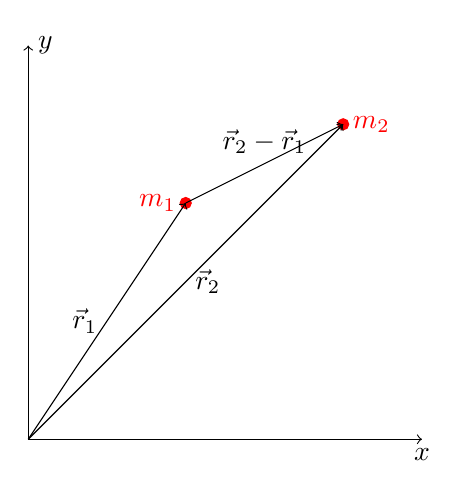
\begin{tikzpicture}
        \draw[black, ->] (0,0) -- (5,0) node[anchor=north]{$x$};
        \draw[black, ->] (0,0) -- (0,5) node[anchor=west]{$y$};

        \filldraw[red] (2,3) circle (2pt) node[anchor=east]{$m_1$};
        \filldraw[red] (4,4) circle (2pt) node[anchor=west]{$m_2$};

        \draw[black, ->] (2,3) -- (4,4) node[anchor=south, midway]{$\vec r_2 - \vec r_1$};
        \draw[black, ->] (0,0) -- (2,3) node[anchor=east, midway]{$\vec r_1$};
        \draw[black, ->] (0,0) -- (4,4) node[anchor=west, midway]{$\vec r_2$};

    \end{tikzpicture}

    \captionof{figure}{Two masses in space}
    \label{fig:gravforce_masses}
\end{center}

We have that the gravitational force is given by

$$
    \vec F = G \frac{ m_1 m_2}{|\vec r_2 - \vec r_1|^2} \hat r
$$

Note that if we put $F = ma$ we get that the acceleration for $m_1$ is

$$
    \vec a = G \frac{m_2}{|\vec r_2 - \vec r_1|^2} \hat r
$$

If we are on the surface of the Earth we can use the approximation $|\vec r_2 - \vec r_1| \approx R$, since the position on the planet is negligible compared to the radius of the planet.

Then we get that the acceleration of any object on the surface of Earth is

$$
    \vec a = - G \frac{M}{R^2} = g \approx \SI{9.81}{\meter \per \second \squared}
$$

\subsection{Examples}

\subsubsection{Example 1}

Consider the very basic case of a still box of mass $m$ on a table.

We have two forces acting on the box: the gravitational force (pulling the box down) and the normal force (keeping the box on the table).

$$
    \vec N = - m \vec g
$$

\subsubsection{Example 2}

Consider two boxes one next to the other on a surface with no friction, one of mass $m_1$ and the other of mass $m_2$.

\begin{center}
    \begin{tikzpicture}
        \draw[black] (0,0) -- (5,0);
        \draw[blue] (2,0) rectangle (3,1) node[midway]{$m_1$};
        \draw[red] (3,0) rectangle (4,3) node[midway]{$m_2$};
    \end{tikzpicture}
\end{center}

Intuitively we can just consider the two boxes as a single object of mass $m_1 + m_2$ but we will solve the problem as if we didn't notice this.

For each body we can draw a \textbf{free body diagram}:

\begin{center}
    \begin{tikzpicture}
        % m_1
        \draw[blue] (-4,0) rectangle (-2,2) node[midway]{$m_1$};

        \draw[black, ->] (-3,0) -- (-3,-1) node[anchor=west, midway]{$-m_1 g$};
        \draw[black, ->] (-3,2) -- (-3,3) node[anchor=west, midway]{$\vec N_1$};
        \draw[black, ->] (-5,1) -- (-4,1) node[anchor=north, midway]{$\vec F$};
        \draw[black, ->] (-2,1) -- (-1,1) node[anchor=north, midway]{$\vec f_1$};

        % m_2
        \draw[red] (4,0) rectangle (6,2) node[midway]{$m_2$};

        \draw[black, ->] (5,0) -- (5,-1) node[anchor=west, midway]{$-m_2 g$};
        \draw[black, ->] (5,2) -- (5,3) node[anchor=west, midway]{$\vec N_2$};
        \draw[black, ->] (3,1) -- (4,1) node[anchor=north, midway]{$-\vec f$};
    \end{tikzpicture}
\end{center}

We know that the normal forces are equal and opposite to the gravitational forces, and since there are no other forces acting in those directions we can cancel them out.

Now we focus on the horizontal direction.
We write the second law for each box:

\begin{align*}
    m_1 a_1 & = F - f \\
    m_2 a_2 & = f
\end{align*}

and

$$
    (m_1 + m_2) a = F
$$

\subsubsection{Example 3}

Consider two boxes connected by a rope.
We can define \textbf{tension} as the force exerted by the rope on the boxes.
By the third law we have that the tension is the same for both boxes.

\section{Class of 15/02/2024}

\subsection{Equivalence principle}

We have two different kind of masses: the \textbf{inertial mass} and the \textbf{gravitational mass}.

The first one is the mass that appears in the second law, the second one is the mass that appears in the gravitational force.

The equivalence principle (proposed by Einstein) states that the two masses are the same.

\subsubsection{Example: elevator}

Consider an elevator which is accelerating upwards with an acceleration $a$.

We have that

$$
    N - m g = m a
$$

Where $N$ is the normal force. We get that $N = m(a + g)$

(Note that we are ignoring tidal forces.)

This principle says that there is no way to distinguish between the two forces, in the example we see how we cannot know if the elevator is accelerating or if the gravitational force is stronger.

\subsection{Harmonic oscillator}

Consider a mass $m$ attached to a spring with spring constant $k$. Let $\Delta x$ be the displacement from the equilibrium position $x_0$. For simplicity we will consider a system with origin in $x_0$. Suppose there is no gravity and no friction.

From the equation of motion we have that

$$
    m a_x = m \dv[2]{t}x(t) = F(t) = - k x(t)
$$

We need to solve the differential equation

$$
    \dv[2]{t}x(t) = - \frac{k}{m} x(t)
$$

\subsubsection{Solving the differential equation}

To solve this we have to find a function that is its own second derivative but with the sign changed.

We can work on the function $e^t$ since it is similar to the result we want to get. We can obtain the minus sign by introducing the imaginary unit $i$.

$$
    \dv[2]{t}e^{i t} = - e^{i t}
$$

Although this would work we have the problem of the dimension of time: when we do a taylor expansion of a $e^t$ we get a number that has dimension $[T] + [T]^2 + \dots$ which is not what we want.

To get rid of the dimension of $t$ we introduce a coefficient $\omega$ with dimension $[T]^{-1}$.

$$
    \dv[2]{t}e^{i \omega t} = - \omega^2 e^{i \omega t}
$$

From complex analysis we know Euler's formula:

$$
    e^{i \omega t} = \cos (\omega t) + i \sin (\omega t)
$$

Now, since we are doing physics here, we want to get rid of the imaginary unit.

We notice that both $\cos(\omega t)$ and $\sin(\omega t)$ solves the equation. When we solve differential equations (we know ?) that the general solution is a linear combination of 2 particular solutions.

$$
    x(t) = A \cos(\omega t) + B \sin(\omega t)
$$

Now we reparametrize the function:

\begin{align*}
    A & = R \cos(\gamma) \\
    B & = R \sin(\gamma)
\end{align*}

We can write the function as

\begin{align*}
    x(t) & = R \cos(\gamma) \cos(\omega t) + R \sin(\gamma) \sin(\omega t)              \\
         & = R \left( \cos(\gamma) \cos(\omega t) + \sin(\gamma) \sin(\omega t) \right) \\
         & = R \cos(\omega t - \gamma)
\end{align*}

\subsubsection{Fixing the constants}

We know that $\omega^2 = \frac{k}{m} \implies \omega = \pm \sqrt{\frac{k}{m}}$.

Now we have to fix the constants $R$ and $\gamma$ and to do so we will use the initial conditions of the system.

\begin{align*}
    x(0) & = x_0 = R \cos(\gamma)        \\
    v(0) & = v_0 = R \omega \sin(\gamma)
\end{align*}

We obtain these results by setting $t = 0$ in the function and in its derivative and exploiting the fact that sine is an even function.

\subsection{Friction}

Friction is quite a complex force that depends on many complex factors. For the purpose of this course we will consider a simple model of friction which describes well enough the behavior we see in real life.

The first thing we notice is that the friction depends on the two surfaces in contact, we will model this through a coefficient $\mu$.

Moreover we see how if we push a mass with a force $F$ the friction will keep the mass still until the force is greater than a certain value, after that threshold the mass will start moving.
We call this value $f_{\text{max}}$ and say that $\norm{f} \leq f_{\text{max}}$.

We also notice that the friction is proportional to the normal force. Combining all the above we get that

$$
    f = \mu N
$$

The direction of this force is opposite to the direction of the force that is trying to move the mass.

Moreover the coefficient $\mu$ changes if the mass is moving or not: if the mass is still we use the static coefficient of friction $\mu_s$, if the mass is moving we use the kinetic coefficient of friction $\mu_k$.

\subsubsection{Example: Inclined plane}

\begin{center}
    \begin{tikzpicture}
        \draw[black] (0,3) -- (5,0);
        \draw[black] (0,0) -- (5,0) node[midway, below]{$b$};
        \draw[black] (0,0) -- (0,3) node[midway, left]{$h$};

        \draw[blue, rotate=59] (2.57,-2) rectangle (4.07,-0.5) node[midway]{$m$};
    \end{tikzpicture}
\end{center}

Consider a mass $m$ on an inclined plane with angle $\theta$.

We have that $\theta = \arctan\left(\frac{h}{b}\right)$.

The gravitational force is always pointing towards $-\hat j$, hence it will try to pull the mass down the plane.

Since the plane is inclined we need to find the two components of the gravitational force in order to find which one is causing the body to move and which one is creating a normal force.

The friction force, then, will be pointing in the opposite direction of motion, hence the opposite direction of the component of the gravitational force that is causing the motion.

We will consider as frame of reference the one that is parallel $\hat u_{\parallel}$ and perpendicular $\hat u_{\perp}$ to the plane.

Consider the forces along each direction:

\begin{itemize}
    \item $\hat u_{\parallel}$:
          Here we have the gravitational force $F_{g\parallel} = mg \sin \theta$ and the friction $f = \mu N$
    \item $\hat u_{\perp}$: Here we have the normal force $N$ and the gravitational force $F_{g\perp} = mg \cos \theta = - N$
\end{itemize}

The body will start moving only after $F_{g\parallel} > f$. Thus

\begin{align*}
    F_{g\parallel} & < f       \\
    mg \sin \theta & < \mu_s N
\end{align*}

We call $\theta_c$ ($\theta$ critical) the angle at which the body starts moving. We can calculate it as follows:

\begin{align*}
    mg \sin \theta_c & = \mu_s N                \\
    mg \sin \theta_c & = \mu_s mg \cos \theta_c \\
    \tan \theta_c    & = \mu_s
\end{align*}

This is very important because in this way we have a way to measure the coefficient of friction.

\section{Class of 19/02/2024 - Exercises}

\begin{warningbox}{Exercises}
    In this class we just solved exercised so I won't report anything here except for important results.
\end{warningbox}

We derived, by solving some exercises, the following relations:

$$
    \frac{\sin \theta_1}{\sin \theta_2} = \frac{v_1}{v_2}
$$

and

$$
    \theta_1 = \theta_2
$$

These are relations that describe the refraction and reflection of light but it's interesting to see how they can be derived from the fact that light travels the fastest path.

\section{Class of 20/02/2024 - Work and energy}

\subsection{Work-energy theorem}

Consider the following equations:

\begin{align*}
    \dv{v}{t}                                 & = a                         \\
    v \dv{v}{t}                               & = a v                       \\
    \frac{1}{2} \dv{v^2}{t}                   & = a \dv{x}{t}               \\
    \frac{1}{2} \int_{v_0}^{v_1} v^2 \dd{}    & = a \int_{x_0}^{x_1} \dd{x} \\
    \frac{1}{2} (v_1^2 - v_0^2)               & = a (x_1 - x_0)             \\
    \frac{1}{2} (v_1^2 - v_0^2)               & = \frac{F}{m} (x_1 - x_0)   \\
    \frac{1}{2} m v_1^2 - \frac{1}{2} m v_0^2 & = F (x_1 - x_0)
\end{align*}


We have seen these equations up to the fifth line but now that we know that $F = m a$ we can write the equation in terms of the force.

Note that this equation does not depend on time.

We define the following from the equation above:

\begin{itemize}
    \item \underline{Work}: $W = F \Delta x$
    \item \underline{Kinetic energy}: $K = \frac{1}{2} m v^2$
\end{itemize}

We get the \textbf{work-energy theorem}:

$$
    \Delta K = W
$$

The unit of energy and work is

$$
    [K] = [W] = [F][L] = [M][L]^2[T]^{-2} = \si{\kilogram \meter \squared \per \second \squared} = \si{\joule}
$$

\subsection{Power}

Moreover we define \textbf{power} as the rate of change of work:

\begin{align*}
    P & = \dv{W}{t}           \\
      & = \dv{t} (F \Delta x) \\
      & = F \dv{x}{t}         \\
      & = F v
\end{align*}


The unit of power is

$$
    [P] = [F][L][T]^{-1} = \si{\kilogram \meter \squared \per \second \cubed} = \si{\watt}
$$

\subsection{Non-constant force}

Note that the relationship we defined above are valid only if the force is constant, otherwise we have to do some extra work.

In fact

\begin{align*}
    \dd{W}          & = F(x) \dd{x}          \\
    \int_0^1 \dd{W} & = \int_0^1 F(x) \dd{x} \\
    W = K_1 - K_0   & = \int_0^1 F(x) \dd{x}
\end{align*}

\subsection{Potential energy}

Assume we know

$$
    F(x) = \dv{x} G(x)
$$

for some function $G(x)$.

We get

$$
    \int_0^1 F(x) \dd{x} = \int_0^1 \dv{G}{x} \dd{x}
$$

We can simplify the differentials and get

$$
    \int_0^1 F(x) \dd{x} = \int_0^1 \dd{G} = G(1) - G(0)
$$

We define the \textbf{potential energy} associated to a force $F$ as

$$
    V = - G
$$

We will use this concept to define the total mechanical energy:

$$
    E = K + V = \text{ const}
$$


\subsubsection{Example: gravitational force}

We know that

$$
    F_g = - m g \hat j = - \dv{V_g}{y}(y) \hat j
$$

We get that the potential is

$$
    V_g(y) = m g y + c
$$

Note that the potential is an artificial construct which cannot be measured directly.
That's why we have the $c$ term: this is a constant we can choose to make the potential zero at some point.

\subsubsection{Example: spring force}

We know that

$$
    F_s(x) = -k (x - x_0) = - \dv{V_s}{x}(x)
$$

We get that the potential is

\begin{align*}
    V_s(x) & = \frac{1}{2} k (x - x_0)^2 + c  \\
           & = \frac{1}{2} k (\Delta x)^2 + c
\end{align*}

\subsection{Non conservative forces}

We will start with an example.

Consider a mass $m$ on a surface with friction attached to a spring.

We write the equation of work:

$$
    (K_1 + \frac{1}{2}kx_1^2) - (K_0 + \frac{1}{2}kx_0^2) = W_{\text{friction}}
$$

This $W_{\text{friction}}$ is the work done by the friction force and it is something like

$$
    W_{\text{friction}} = \int_0^1 f(x, \ldots) \dd{x}
$$

Friction is a complex force that depends on many factors, hence we cannot integrate it that easily. We recall that in our model $\vec f = \mu_d \vec N$, thus

\begin{align*}
    W_{\text{friction}} & = \int_0^1 \mu_d mg \dd{x} \\
                        & = \mu_d mg (x_1 - x_0)     \\
                        & < 0
\end{align*}

We see that when we introduce friction we lose energy, hence we call friction a \textbf{non-conservative force}.

\subsubsection{Example}

Consider a mass $m$ on a surface with friction attached to a spring.

We want to find $x_1$ given $x_0$ and that $K_0 = K_1 = 0$ (we want to find the position at which $m$ stops).

If we take the equation from above and remove the kinetic energies we get

\begin{align*}
    \frac{1}{2} k x_1^2 - \frac{1}{2} k x_0^2 & = - \mu_d m g (x_1 - x_0) \\
    \frac{1}{2} k (x_1^2 - x_0^2)             & = - \mu_d m g (x_1 - x_0) \\
    \frac{1}{2} k (x_1 - x_0)(x_1 + x_0)      & = - \mu_d m g (x_1 - x_0) \\
\end{align*}

and

$$
    (x_1 - x_0) \left( \frac{1}{2} k (x_1 + x_0) + \mu_d m g \right) = 0
$$

This equation tells us some interesting facts:
we get that $m$ will be still if $x_1 = x_0$ or if $x_1 = -x_0$ minus some factor that depends on the friction.

\subsection{Dynamical system}

Consider the problem of finding the position of a point knowing just the forces acting on it.

We have seen this problem before by using a second order differential equation, but we can also solve it by using the concept of potential energy.

We have that

\begin{align*}
    E                  & = \frac{1}{2} m \left( \dv{x}{t} \right) + V(x) = \text{ const} \\
    \implies \dv{x}{t} & = \pm \sqrt{\frac{2}{m} (E - V(x))}
\end{align*}

\begin{bluebox}{Sidenote: separable differential equations}
    To complete this problem we need to solve a differential equation of the form

    $$
        \dv{x}{t} = f(x) g(t)
    $$

    This type of equation is called \textbf{separable} and it's one of the few types of differential equations that can be solved analytically.

    We can solve it by separating the variables and integrating both sides:

    \begin{align*}
        \dv{x}{t}                         & = f(x) g(t)        \\
        \implies \int \frac{\dd{x}}{f(x)} & = \int g(t) \dd{t}
    \end{align*}

    Remember to choose the same bounds for both integrals.
\end{bluebox}

We identify that $\dv{x}{t} = f(x)g(t)$ where $f(x) = \pm \sqrt{\frac{2}{m} (E - V(x))}$ and $g(t) = 1$.
Now we can solve the separable differential equation:

$$
    \pm \int_0^1 \frac{\dd{x}}{\sqrt{\frac{2}{m} (E - V(x))}} = \int_0^1 \dd{t} = t
$$

\section{Class of 22/02/2024}

\subsection{Equilibrium}

An mass is in equilibrium when $F = 0$.
We also know that $F = -\dv{V}{x}$.

Moreover we can study the \textbf{stability} of the equilibrium by looking to what happens to the force when we move the mass a little bit from the equilibrium:
we say that the equilibrium is \textbf{stable} if the force is directed towards the equilibrium and \textbf{unstable} if the force is directed away from the equilibrium. Hence we have stability if $V''(x) > 0$.

Consider the following situation:
the mass is converting its kinetic energy into potential energy; it is approaching a point of unstable equilibrium $x_e$ and it has just enough energy $E$ to reach it.
We want to calculate the time it takes to reach the equilibrium.

First we need to compute $V(x_e + \delta x)$, we can do so by using a Taylor expansion.

Then we consider the bound of integration $x_0 = x_e + \delta x_0$ and $x_1 = x_e + \delta x_1$ and use the formula we saw in the last class to find the time.

$$
    \Delta t = \pm \int_{x_e + \delta x_0}^{x_e + \delta x_1} \frac{\dd{x}}{\sqrt{\frac{2}{m} (E - V(x_e + \delta x))}}
$$

Then the best approach to try to solve this integral is to use a Taylor expansion of $V$, substitute $u = \delta x$ and shift the bounds of integration.

If we are lucky we might be able to solve this integral analytically, surely it's easier to solve this than the second order differential equation.

\subsection{Work and energy in 2D}

We have that the total mechanical energy is conserved if the forces are conservative.

A force is conservative if it only depends on starting and ending points and not on the path taken. In 1D this is easy to see, it's a bit more difficult in 2D and 3D.

In 1D we have that

$$
    f(x + \dd{x}) - f(x) = \dd{f} = f'(x) \dd{x}
$$

In higher dimensions we have to use partial derivatives.

\subsubsection{Calculus review: partial derivatives}

Consider a function $f(x, y)$, we have that

\begin{align*}
    \pdv{f}{x} & = \lim_{\Delta x \to 0} \frac{f((x + \Delta x), y) - f(x, y)}{\Delta x} \\
    \pdv{f}{y} & = \lim_{\Delta y \to 0} \frac{f(x, (y + \Delta y)) - f(x, y)}{\Delta y}
\end{align*}

where $\pdv{f}{x}$ and $\pdv{f}{y}$ are called \textbf{partial derivatives} of $f$ with respect to $x$ and $y$.
This means that we fix one variable and we take the derivative with respect to the other.

Partial derivatives represent the variation of the function along just one direction, now we have to find what is the total variation $\dd{f}$ of the function.

Consider the two possible paths $(A)$ and $(B)$ to go from $(x, y)$ to $(x + \dd{x}, y + \dd{y})$ as in Figure (\ref{fig:partial_derivatives}):

\begin{figure}[H]
    \centering
    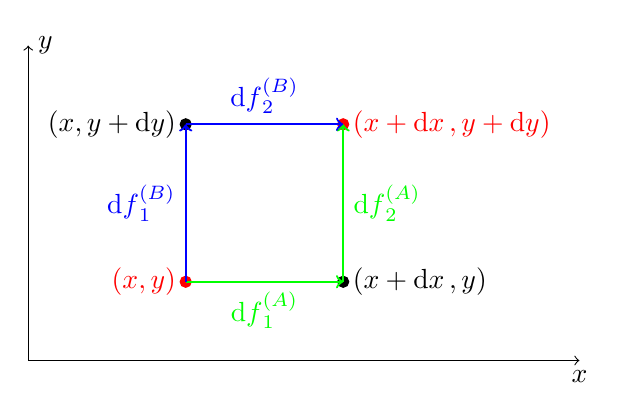
\begin{tikzpicture}
        \draw[black, ->] (-1,0) -- (6,0) node[anchor=north]{$x$};
        \draw[black, ->] (-1,0) -- (-1,4) node[anchor=west]{$y$};

        \filldraw[red] (1,1) circle (2pt) node[anchor=east]{$(x, y)$};
        \filldraw[red] (3,3) circle (2pt) node[anchor=west]{$(x + \dd{x}, y + \dd{y})$};
        \filldraw[black] (1,3) circle (2pt) node[anchor=east]{$(x, y + \dd{y})$};
        \filldraw[black] (3,1) circle (2pt) node[anchor=west]{$(x + \dd{x}, y)$};

        \draw[thick, green, ->] (1,1) -- (3,1) node[anchor=north, midway]{$\dd{f}_1^{(A)}$};
        \draw[thick, green, ->] (3,1) -- (3,3) node[anchor=west, midway]{$\dd{f}_2^{(A)}$};
        \draw[thick, blue, ->] (1,1) -- (1,3) node[anchor=east, midway]{$\dd{f}_1^{(B)}$};
        \draw[thick, blue, ->] (1,3) -- (3,3) node[anchor=south, midway]{$\dd{f}_2^{(B)}$};
    \end{tikzpicture}

    \caption{Possible paths to go from $(x, y)$ to $(x + \dd{x}, y + \dd{y})$}
    \label{fig:partial_derivatives}
\end{figure}

\begin{itemize}
    \item For $(x, y) \to (x + \dd{x}, y) \to (x + \dd{x}, y + \dd{y})$ we have

          \begin{align*}
              \dd{f}_1^{(A)} & = \pdv{f(x,y)}{x} \dd x          \\
              \dd{f}_2^{(A)} & = \pdv{f(x + \dd x, y)}{y} \dd y
          \end{align*}

    \item For $(x, y) \to (x, y + \dd{y}) \to (x + \dd{x}, y + \dd{y})$ we have

          \begin{align*}
              \dd{f}_1^{(B)} & = \pdv{f(x,y)}{y} \dd y          \\
              \dd{f}_2^{(B)} & = \pdv{f(x, y + \dd y)}{x} \dd x
          \end{align*}
\end{itemize}

We now want to prove that

$$
    \dd{f}_1^{(A)} + \dd{f}_2^{(A)} \stackrel{?}{=} \dd{f}_1^{(B)} + \dd{f}_2^{(B)}
$$

Now we note that the terms $\dd{f}_2^{(A)}$ and $\dd{f}_2^{(B)}$ are partial derivatives at a mid point that depends on $\dd{x}$ and $\dd{y}$ respectively,
if we use a Taylor expansion on those we get the following results:

\begin{align*}
    \dd{f_2}^{(A)} = \pdv{f(x + \dd{x}, y)}{y} \dd{y} & = \pdv{f(x, y)}{y} \dd{y} + \pdv{x} \left( \pdv{f(x, y)}{y} \dd{y} \right) \dd{x} \\
                                                      & = \pdv{f(x, y)}{y} \dd{y} + \pdv{f(x, y)}{x}{y} \dd{x} \dd{y}                     \\
    \dd{f_2}^{(B)} = \pdv{f(x, y + \dd{y})}{x} \dd{x} & = \pdv{f(x, y)}{x} \dd{x} + \pdv{y} \left( \pdv{f(x, y)}{x} \dd{x} \right) \dd{y} \\
                                                      & = \pdv{f(x, y)}{x} \dd{x} + \pdv{f(x, y)}{y}{x} \dd{y} \dd{x}
\end{align*}

(Note that Taylor expansions of functions of multiple variables have not been covered yet in analysis 2, hence we will not prove the above results.
If you're curious ChatGPT is your friend.)

Now if we substitute these results in the equation we want to prove we can simplify a lot to get that

$$
    \pdv{f(x, y)}{x}{y} \dd{x} \dd{y} \stackrel{?}{=} \pdv{f(x, y)}{y}{x} \dd{y} \dd{x}
$$

This result says that the mixed partial derivatives are equal, which is true for most functions we will encounter.

\subsubsection{Application to energy conservation}

Now that we know how to use partial derivatives we can show that the kinetic energy is

\begin{align*}
    K & = \frac{1}{2} m v^2                        \\
      & = \frac{1}{2} m \norm{\vec{v}}^2           \\
      & = \frac{1}{2} m \left(v_x^2 + v_y^2\right) \\
\end{align*}

And knowing that power is the rate of change of work we can write the work done by a force as

\begin{align*}
    P = \dv{K}{t} & = \frac{1}{2}m \dv{t} \left(v_x^2 + v_y^2\right)                  \\
                  & = \frac{1}{2}m \left(\dv{t} v_x^2 + \dv{t} v_y^2\right)           \\
                  & = \frac{1}{2}m \left(2 v_x \dv{v_x}{t} + 2 v_y \dv{v_y}{t}\right) \\
                  & = m (v_x a_x + v_y a_y)                                           \\
                  & = m v_x a_x + m v_y a_y                                           \\
                  & = F_x v_x + F_y v_y                                               \\
                  & = \vec F \cdot \vec v
\end{align*}

Therefore we have that

$$
    \dv{W}{t} = \vec F \cdot \vec v = \vec F \cdot \dv{\vec r}{t}
$$

This result is useful to calculate the work done by a force along a path:
knowing the force and the path we can use a path integral to get the result.
(Path integrals have been explained briefly in today's analysis 2 lecture.)

$$
    W = \int_{\gamma} F(\vec{r}) \cdot \dd{\vec{r}}
$$

Note that from this result we see that there can exist non-zero forces that do no work:
if the direction of the force is orthogonal to the direction of the path then the work is zero.

\subsection{Conservative forces in 2D}

Despite all the effort we put in the calculus section above to show that the mixed partial derivatives are equal is actually only valid for infinitesimal variations of the function.
In fact, in the general case of discrete variations of the function this is not true.

In 1D it was easy to show that every force (except for friction) is conservative, but in 2D and 3D this is not true:
if we just consider 2D, for example, there are infinitely many ways to get from a point to another, and it's easy so see that the work done by a force can depend on the path taken.
If you are not convinced you can read section 6.4 of the book which contains nice examples and more verbose explanations.

To summarize, in $d \geq 2$ we cannot assume that a force is conservative. In fact, in general, we have that

$$
    \int_{\gamma_A} \vec{F}(\vec{r}) \cdot \dd \vec{r} \neq \int_{\gamma_B} \vec{F}(\vec{r}) \cdot \dd \vec{r} \ne V(\vec{r}_A) - V(\vec{r}_B)
$$

\subsubsection{Contructing a conservative force}

Even though we cannot assume that a force is conservative we have a way to construct one.

We choose a $V(x, y)$ such that

$$
    \vec{F} = \left( - \pdv{V}{x}, - \pdv{V}{y} \right) = -\vec{\nabla} V
$$

where $\vec{\nabla} = \left( \pdv{x}, \pdv{y} \right)$ is the \textbf{gradient} operator. (See analysis 2.)

Then

\begin{align*}
    \int_\gamma \vec{F} \cdot \dd{\vec{r}} & = \int_\gamma \left( -\pdv{V}{x}, -\pdv{V}{y} \right) \cdot (\dd{x}, \dd{y}) \\
                                           & = - \int_\gamma \pdv{V}{x} \dd{x} + \pdv{V}{y} \dd{y}                        \\
                                           & = - \int_\gamma \dd{V}                                                       \\
                                           & = V(\vec{r}_A) - V(\vec{r}_B)
\end{align*}

and we obtain the result we wanted.

\section{Class of 23/02/2024 - Gravitation and Kepler's laws}

\subsection{A criterion for conservative forces}

In the last class we have seen that if we have $f(x, y, z)$ and we want to move to $\dd{\vec r} = (\dd{x}, \dd{y}, \dd{z})$ we can write the differential as

\begin{align*}
    \dd{f} & = f(x + \dd{x}, y + \dd{y}, z + \dd{z}) - f(x, y, z)        \\
           & = \pdv{f}{x} \dd{x} + \pdv{f}{y} \dd{y} + \pdv{f}{z} \dd{z} \\
           & = \vec{\nabla} f \cdot \dd{\vec{r}}
\end{align*}

Therefore to have a conservative force we need to have a potential $V(x, y, z)$ such that $\vec{F} = -\vec{\nabla} V$.

Note that $\int_\gamma = -\int_{-\gamma}$, thus if a force is conservative, if we take a path and then go back to the starting point we will get that the total work done is zero. We say $\oint_\gamma \vec{F} \cdot \dd{\vec{r}} = 0$.

We can also derive a criterion to check if a force is conservative without computing integrals:

\begin{align*}
                                          & \pdv{F_x}{y} = \pdv{F_y}{x} \\
    \vec{F} \text{ is conservative } \iff & \pdv{F_x}{z} = \pdv{F_z}{x} \\
                                          & \pdv{F_y}{z} = \pdv{F_z}{y}
\end{align*}

\subsubsection{Kinetic energy must create a conservative force}

We know that
$$
    E = \frac{1}{2} m v^2 + V(\vec{r}) = \text{ const}
$$

Since $E$ and we want a conservative $V$ we can write

\begin{align*}
    \dv{E}{t} = 0 & = \dv{t} \left( \frac{1}{2} m v^2 + V(\vec{r}) \right)                                                              \\
                  & = m \vec{v} \cdot \dv{\vec{v}}{t} + \left(\pdv{V}{x} \dv{x}{t} + \pdv{V}{y} \dv{y}{t} + \pdv{V}{z} \dv{z}{t}\right) \\
                  & = m \vec{v} \cdot \vec{a} + \vec{\nabla} V \cdot \vec{v}                                                            \\
                  & = \vec{F} \cdot \vec{v} + \vec{\nabla} V \cdot \vec{v}                                                              \\
                  & = \vec{v}\left(\vec{F} + \vec{\nabla} V\right) = 0                                                                  \\
\end{align*}

\subsection{Gravitational force}

Before starting with Kepler's laws we need to describe better the gravitational force.

We will derive the law of gravitation from the laws of motion.

We know the following facts:

\begin{enumerate}
    \item From Galileo we know that all bodies fall with the same acceleration.
          We also know that $F = ma$ then $g = \frac{F}{m}$, therefore $F \propto F_0 m$.
    \item Because of the action-reaction principle we have that $F \propto m M$.
    \item Newton also found out that the force that causes the apple to fall is the same force that keeps the moon in orbit.
          Then $F \propto r^{-2}$.
\end{enumerate}

We can combine these facts to get that

$$
    F = - G \frac{m M}{r^2}
$$

A more detailed derivation of this result can be found in the book.

We will now discuss the unit of $G$.
We have

$$
    [G] = [F][M]^{-2}[L]^2 = \si{\newton \meter \squared \per \kilogram \squared} = \si{\meter \cubed \per \kilogram \per \second \squared}
$$

Moreover we find that $G$ is very small, in fact $G = 6.67 \times 10^{-11} \si{\newton \meter \squared \per \kilogram \squared}$.

This is a very small number, in fact, compared to, for example, the electric force, the gravitational force $10^{36}$ times weaker.

\subsubsection{Principle of superposition}

Consider a mass $m$ at a distance $d$ from a rod of mass $M$ of uniform density.

\begin{figure}[H]
    \centering
    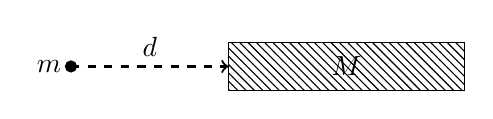
\begin{tikzpicture}
        \filldraw[black] (-2, 0) circle (2pt) node[anchor=east]{$m$};

        \draw[pattern=north west lines, pattern color=black] (0, -0.3) rectangle (3, 0.3) node[midway]{$M$};

        \draw[black, dashed, thick, ->] (-2, 0) -- (0, 0) node[midway, above]{$d$};
    \end{tikzpicture}

    \caption{Mass $m$ at a distance $d$ from a rod of mass $M$}
    \label{fig:mass_rod}
\end{figure}

We can write $M = \int_0^L \rho(x) \dd{x} = \rho L = \frac{M}{L}$.

Then the gravitational force is

\begin{align*}
    \vec F & = - G m \int_0^L \frac{\rho(x)}{{\dd{} x}^2}  \dd{x} \hat i                   \\
           & = - G \frac{m M}{L} \int_0^L \frac{1}{{\dd{} x}^2}  \dd{x} \hat i             \\
           & = - G \frac{m M}{L} \left[ - \frac{1}{\dd{} + x} \right]_0^L \hat i           \\
           & = G \frac{m M}{L} \left( \frac{1}{L + \dd{}} - \frac{1}{\dd{}} \right) \hat i \\
           & = -G \frac{m M}{\dd{} (\dd{} + L)} \hat i
\end{align*}

For a \textbf{sphere} we have to integrate along all the points of the sphere, if we solve the 3D integral we get that it is equivalent to considering all the mass at the center of the sphere.

Consider another case of a mass $m$ at the center of a \textbf{shell} of mass $M$. We see that even if $m$ is not at the very center of the shell the force is still 0.

Consider a cone passing through $m$ and intersecting the shell in two circles of mass $\dd{M_1}$ and $\dd{M_2}$. If $\theta$ is very small the radius of the circle is just $r \dd{\theta}$.

Then

\begin{align*}
    \dd{M_1} & = \rho \dd{A_1} = \rho \pi (r \dd{\theta})^2 \\
    \dd{M_2} & = \rho \dd{A_2} = \rho \pi (r \dd{\theta})^2
\end{align*}

Then we notice that $\dv{M_1}{M_2} = \frac{R_1^2}{R_2^2}$. We could continue this reasoning and complete the proof of the \textbf{shell theorem} but we will stop here.
What we saw it's enough to understand that the force is 0 even if $m$ is not at the center of the shell.

\subsection{Kepler's laws}

These laws have been derived by Kepler but this was only possible thanks to the observations of Brahe.

\begin{enumerate}
    \item Planets follow elliptical orbits
    \item Equal areas are swept in equal times
    \item $T^2 / a^3 = \text{ const}$ where $T$ is the period of the orbit and $a$ is the semi-major axis of the orbit.
\end{enumerate}

For planet Earth we know that $T = 365 \si{day} = 3.2 \times 10^7 \si{s}$ and $a = 1.5 \times 10^{11} \si{m}$, hence we can calculate the constant for the third law to be $3.5 \times 10^{-19} \si{s^2/m^3}$.

Kepler found these laws empirically, but Newton wanted to derive them from his laws. We will now follow Newton's steps and derive Kepler's laws starting from the laws of motion.

We will not derive them in order, we will start with the second law.

\subsubsection{Second Kepler's law}

We have

$$
    m \dv[2]{\vec r}{t} = \vec F = - G \frac{m M}{r^2} \hat r
$$

For this kind of task it is useful to work with polar coordinates, we have

\begin{align*}
    \dv{\hat r}{t}       & = \dv{\theta}{t} \hat \theta \\
    \dv {\hat \theta}{t} & = - \dv{\theta}{t} \hat r
\end{align*}

We can now start computing the second derivative of $\vec r$.

\begin{align*}
    \dv{t} \vec{r} = \dv{t} (r \hat r) & = \dv{r}{t} \hat r + r \dv{\hat r}{t}                                                                                                            \\
    \dv{t}\left(\dv{\vec{r}}{t}\right) & = \dv{t}\left(\dv{r}{t} \hat r + r \dv{\hat r}{t}\right)                                                                                         \\
                                       & = \dv[2]{r}{t} \hat r + \dv{r}{t} \dv{\hat r}{t} + r \dv[2]{\hat r}{t} + r \dv{\theta}{t} \dv{\hat \theta}{t}                                    \\
                                       & = \dv[2]{r}{t} \hat r + \dv{r}{t} \dv{\theta}{t} \hat \theta + r \dv[2]{\theta}{t} \hat \theta - r \left(\dv{\theta}{t}\right)^2 \hat r          \\
                                       & = \left(\dv[2]{r}{t} - r \left(\dv{\theta}{t}\right)^2\right) \hat r + \left(2 \dv{r}{t} \dv{\theta}{t} + r \dv[2]{\theta}{t}\right) \hat \theta
\end{align*}

Now we can apply the equation to both directions separately:

\begin{itemize}
    \item $\hat r$ direction:

          \begin{align*}
              m \left(\dv[2]{r}{t} - r \left(\dv{\theta}{t}\right)^2\right) & = - G \frac{m M}{r^2} \\
              \dv[2]{r}{t} - r \left(\dv{\theta}{t}\right)^2                & = - G \frac{M}{r^2}
          \end{align*}
    \item $\hat \theta$ direction: there is no force in this direction, hence
          $$
              2 \dv{r}{t} \dv{\theta}{t} + r \dv[2]{\theta}{t} = 0
          $$
\end{itemize}

From the $\hat \theta$ direction, by multiplying both sides by $r$ and applying the chain rule, we get

\begin{align*}
    2 r \dv{r}{t} \dv{\theta}{t} + r^2 \dv[2]{\theta}{t} & = 0 \\
    \dv{t}(r^2) \dv{\theta}{t} + r^2 \dv[2]{\theta}{t}   & = 0 \\
    \dv{t}(r^2 \dv{\theta}{t})                           & = 0
\end{align*}

We define the \textbf{angular momentum} as $L = r^2 \dv{\theta}{t}$.
We see that since its derivative is 0 is is constant in time.

We can now look at the problem of the areas covered in the same time.
We will use the sine rule to calculate the area as follows:

\begin{align*}
    \dd{A} & = \frac{1}{2} \norm{\vec r} \norm{\vec{r} + \dd{\vec{r}}} \sin \dd{\theta} \\
           & \sim \frac{1}{2} \norm{\vec r} \norm{\vec{r} + \dd{\vec{r}}} \dd{\theta}   \\
           & \sim \frac{1}{2} r^2 \dd{\theta}                                           \\
\end{align*}

Therefore, if we take the derivatives in terms of $t$ we get
$$
    \dv{A}{t} = \frac{1}{2} \left(r^2 \dv{\theta}{t}\right)
$$

which we know is constant as we have seen before.

\section{Class of 26/02/2024 - Kepler's laws continued}

\subsubsection{Conservation of angular momentum}

In the last class we saw that the angular momentum

$$
    L = r^2 \dv{\theta}{t}
$$

is constant in time. This is a very important result called the \textbf{conservation of angular momentum}.

\subsection{Kepler's laws}

\subsubsection{First Kepler's law}

Most of the heavy lifting has been done in the last class, we just need to finish the proof.

For the sake of brevity we will consider the simper case of a circular orbit, hence $r = \text{const}$.

We start with our usual $ma = F_g$

\begin{align*}
    % m r \dv[2]{\theta}{t} & = - G \frac{m M}{r^2} \hat r \\
    m a_c         & = G \frac{m M}{r^2} \\
    \frac{v^2}{r} & = G \frac{M}{r^2}   \\
    v^2 r         & = G M
\end{align*}

and we have a circular motion with speed $v$ which depends on the radius of the orbit.

\subsubsection{Third Kepler's law}

This proof is also very simple once we know the equations above.

Now remember that $\omega = \frac{2 \pi}{T}$, therefore, substituting

\begin{align*}
    v^2 r                              & = G M                 \\
    \omega^2 r^3                       & = G M                 \\
    r^3 \left(\frac{2 \pi}{T}\right)^2 & = G M                 \\
    \frac{T^2}{r^3}                    & = \frac{4 \pi^2}{G M}
\end{align*}

\subsection{Gravitational potential energy}

By using the fact that $\hat r = \frac{\vec r}{r}$ we can write the force as

\begin{align*}
    \vec F_g (\vec r) & = - G \frac{m M}{r^2} \hat r                         \\
                      & = G \frac{m M}{r^3} \vec r                           \\
                      & = G \frac{m M}{r^3} (x \hat i + y \hat j + z \hat k) \\
\end{align*}

and we claim that

$$
    % V_g(x, y, z) = - G \frac{m M}{\sqrt{x^2 + y^2 + z^2}} = V(\sqrt{x^2 + y^2 + z^2}) = 
    V(r) = - G \frac{m M}{r}
$$

Indeed if we calculate the gradient of $V$ we get

\begin{align*}
    - \vec \nabla V_g & = \dv{V}{r} \left(\pdv{r}{x},\pdv{r}{y},\pdv{r}{y} \right)                                  \\
                      & = - G \frac{m M}{r^2} \left(\pdv{r}{x},\pdv{r}{y},\pdv{r}{y} \right) \sqrt{x^2 + y^2 + z^2} \\
                      & = - G \frac{m M}{r^2} \frac{(x, y, z)}{\sqrt{x^2 + y^2 + z^2}}                              \\
                      & = - G \frac{m M}{r^2} \frac{\vec r}{r}                                                      \\
                      & = - G \frac{m M}{r^2} \hat r                                                                \\
                      & = \vec F_g
\end{align*}

(Despite all of this notation being very confusing, we are just taking derivatives of $V$. We are taking 3 derivatives at once, but if you solve them one by one you get the same result. See the book at page 114 if you are confused.)

\subsubsection{On the surface of Earth}

We now have to choose a point of zero potential. This is not a trivial task, especially if we consider that just plugging in the equations we had before doesn't work:

$$
    - \frac{G m M}{R + \delta r} = m g \delta r = \frac{G M m}{R^2} \delta r
$$

note that $\delta r = h$: this is just a matter of notation to help emphasize that $\delta r$ is very small.
We obtain this equality by substituting the $g = \frac{GM}{R^2}$, as we found before, in the standard $mgh$ formula, but surely it cannot be right, since the sign are inverted.

Since on the surface of Earth $\delta r$ is very small we can perform a Taylor expansion to get

\begin{align*}
    V(R + \delta r) & = - G \frac{m M}{R + \delta r}                                            \\
                    & = - G \frac{m M}{R (1 + \frac{\delta r}{R})}                              \\
                    & \sim - G \frac{m M}{R} (1 - \frac{\delta r}{R}) + \mathcal{O}(\delta r^2) \\
                    & = - G \frac{m M}{R} + G \frac{m M}{R^2} \delta r                          \\
                    & = V(R) + m g \delta r
\end{align*}

Note that this is only a good approximation only if $\delta r$ is small.

\subsubsection{Energy conservation for planets}

We have that

\begin{align*}
    E & = \frac{1}{2} m v^2 - G \frac{m}{M}           \\
      & = \frac{1}{2} m \frac{G M}{r} - G \frac{m}{M} \\
      & = - \frac{G m M}{2 r} < 0
\end{align*}

This is called a bound state.

If we fix $E_0$ and we want to $\max r$ we need to solve for $v = 0$ and we get

\begin{align*}
    E_0 & = - \frac{G m M}{2 r}   \\
    r   & = - \frac{G m M}{2 E_0}
\end{align*}

We could also reverse the problem and ask for the minimum $v$ to \say{escape the gravitational field} (that is $E = 0$).

\begin{align*}
    E & = \frac{1}{2} m v^2 - G \frac{mM}{R} = 0 \\
    v & = \sqrt{\frac{2 G M}{R}}
\end{align*}

Moreover we could even calculate the radius such that a mass $M$ would have more gravitational energy than the speed of light.

$$
    R^* < \frac{2 G M}{c^2}
$$

This is called the Schwarzschild radius and it is the radius of the event horizon of a black hole.

\section{Class of 27/02/2024 - Multi-particle dynamics}

Consider a 1D system of 2 particles connected by a spring.
This is already a quite hard problem with a very complex motion.

\subsection{Center of mass}

We start by writing Newton's second law for both particles.

\begin{align*}
    m_1 \dv[2]{x_1}{t} & = F_{12} + F_{1 \text{ext}} \\
    m_2 \dv[2]{x_2}{t} & = F_{21} + F_{2 \text{ext}}
\end{align*}

we also know that $F_{21} = - F_{12}$. We can now sum up the two equations to get

$$
    m_1 \dv[2]{x_1}{t} + m_2 \dv[2]{x_2}{t} = F_{1 \text{ext}} + F_{2 \text{ext}}
$$

We can now generalize this to $N$ particles.

\begin{align*}
    \dv[2]{t} \sum_{i = 1}^N m_i x_i & = \sum_{i = 1}^N F_{i \text{ext}}                             \\
                                     & = \sum_{i = 1}^N m_i \dv[2]{x_i}{t}                           \\
                                     & = M \dv[2]{t} \left( \frac{\sum_{i = 1}^N m_i x_i}{M} \right) \\
                                     & = M \dv[2]{x_{cm}}{t}
\end{align*}

where

$$
    x_{cm} = \frac{1}{M} \sum_{i = 1}^N m_i x_i
$$

is the center of mass of the system, that is the weighted average of the positions with respect to the masses.

Moreover, the computation of the center of mass can be done in steps, by considering 2 masses at the time. This can be useful to simplify the computation.

\subsubsection{Center of mass of a rod}

First we consider an uniform rod of length $L$.
We have

$$
    M = \int_0^L \rho(x) \dd{x} = \rho L
$$

because the density $\rho$ is constant.

To find the center of mass we can use

$$
    x_{cm} = \frac{1}{M} \int_0^L \dd{m}(x) x = \frac{L}{2}
$$

This was quite trivial to solve. Things will get more complicated once we consider a non-constant density.

Let $\rho(x) = \rho_0 x$. We have

\begin{align*}
    x_{cm} & = \frac{\int_0^L \dd{m}(x) x}{M}       \\
           & = \frac{\int_0^L \rho(x) \dd{x} x}{M}  \\
           & = \frac{\int_0^L \rho_0 x^2 \dd{x}}{M} \\
           & = \frac{\rho_0}{M} \frac{L^3}{3}       \\
\end{align*}

Moreover we can find the total mass with

$$
    M = \int_0^L \rho(x) \dd{x} = \int_0^L \rho_0 x \dd{x} = \rho_0 \frac{L^2}{2}
$$

and $\rho_0 = \frac{2M}{L^2}$.

If we substitute this result in the equation for $x_{cm}$ we get

$$
    x_{cm} = \frac{L}{3}
$$

\subsubsection{Center of mass of a triangle}

Consider a triangle as such:

\begin{figure}[H]
    \centering
    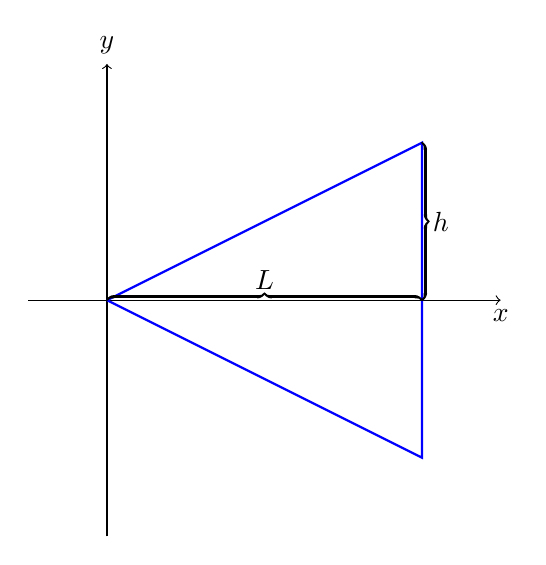
\begin{tikzpicture}
        \draw[black, ->] (-1,0) -- (5,0) node[anchor=north]{$x$};
        \draw[black, ->] (0,-3) -- (0,3) node[anchor=south]{$y$};

        \draw[blue, thick] (0,0) -- (4,2) -- (4,-2) -- (0,0);

        \draw[black, very thick, decorate, decoration={calligraphic brace, mirror}] (4,0) -- (4,2) node[midway, anchor=west]{$h$};
        \draw[black, very thick, decorate, decoration={calligraphic brace}] (0,0) -- (4,0) node[midway, anchor=south]{$L$};
    \end{tikzpicture}
    \caption{Center of mass of a triangle}
    \label{fig:cm_triangle}
\end{figure}

In this example, because of symmetry, we see that $y_{cm} = 0$.
Moreover, we can write

\begin{align*}
    y(x)                      & = \frac{h}{L} x         \\
    \dd{A}(x) = 2 y(x) \dd{x} & = \frac{2h}{L} x \dd{x} \\
\end{align*}

Then, since the density is constant, we have

$$
    \dd{m}(x) = \rho \dd{A}(x) = \rho \frac{2h}{L} x \dd{x}
$$

and the center of mass is

\begin{align*}
    x_{cm} & = \frac{\int_0^L \dd{m}(x) x}{M}                  \\
           & = \frac{\int_0^L \rho \frac{2h}{L} x^2 \dd{x}}{M} \\
           & = \frac{2 \rho h}{ML} \frac{L^3}{3}               \\
\end{align*}

then, since $M = \rho A = \rho h L$ and $\rho = \frac{M}{hL}$ we get

$$
    x_{cm} = \frac{L}{3}
$$

\subsection{Conservation of momentum}

We have

\begin{align*}
    \vec{p}_{cm} = M \dv{\vec{r}_{cm}}{t} & = \sum_{i = 1}^N m_i \dv{\vec{r}_i}{t} \\
                                          & = \sum_{i = 1}^N \vec{p}_i
\end{align*}

Moreover, we can consider the fundamental law of motion:

$$
    \vec{F}_{\text{ext}} = \dv{\vec{p}_{cm}}{t}
$$

Therefore if there are no external forces the total momentum is conserved.

\section{Class of 29/02/2024}

Consider the motion of a rocket.
At time $t_0$ the rocket has mass $m + \delta m$ and velocity $v$.
At time $t_1$ the propeller gets activated and the rocket has mass $m$ and velocity $v + \delta v$, while the propeller has mass $\delta m$ and velocity $v + \delta v + v_r$.

By conservation of quantity of motion we have

\begin{align*}
    (m + \delta m) v & = m (v + \delta v) + \delta m (v + \delta v + v_r)         \\
                     & \implies \delta m (\delta v + v_r) + m \delta v = 0        \\
                     & \implies \delta m \delta v + \delta m v_r + m \delta v = 0
\end{align*}

Now we approximate by saying that $\delta m \delta v \approx 0$ and we get

$$
    \frac{\delta m}{m} = - \frac{\delta v}{v_r}
$$

Let $\dd{m}$ be the change of mass of the rocket. We get that $\dd{m} = - \delta m$.

We can now substitute and, since $v_r < 0$, we can write it as $v_r = - \abs{v_r}$.

$$
    \frac{\dd{m}}{m} = -\frac{\dd{v}}{\abs{v_r}}
$$

Now we can integrate and get

\begin{align*}
    - \int \frac{\dd{m}}{m} & = \int \frac{\dd{v}}{\abs{v_r}} \\
    \log \frac{m(t)}{m}     & = \frac{v(t) - v_0}{\abs{v_r}}
\end{align*}

\subsection{Collisions}

The only thing we know is that the total momentum is conserved. Thus

$$
    p_{cm} = m_1 v_1 + m_2 v_2 = p_1 + p_2 = m_1 v_1' + m_2 v_2' = p_1' + p_2'
$$

This is not enough to solve the problem, but we can specify additional constraint:

\begin{enumerate}[label=\Alph*)]
    \item Inelastic collision: $v'_1 = v_2'$, the two masses stick together
    \item Elastic collision: $E_1 = E_2$, the total energy is conserved
\end{enumerate}

\subsubsection{Inelastic collision}

We have

\begin{align*}
    m_1 v_1 + m_2 v_2 & = (m_1 + m_2) v'                      \\
    v'                & = \frac{m_1 v_1 + m_2 v_2}{m_1 + m_2} \\
    \dv{t} x_{cm}     & = v_{cm}
\end{align*}

We immediately see that here energy is not conserved.

\subsubsection{Elastic collision}

We have

\begin{align*}
     & \begin{cases}
           m_1 v_1 + m_2 v_2 = m_1 v_1' + m_2 v_2' \\
           \cancel{\frac{1}{2}} m_1 v_1^2 + \cancel{\frac{1}{2}} m_2 v_2^2 = \cancel{\frac{1}{2}} m_1 (v_1')^2 + \cancel{\frac{1}{2}} m_2 (v_2')^2
       \end{cases} \\
     & \begin{cases}
           m_1(v_1 - v_1') = m_2(v_2' - v_2) \\
           m_1 (v_1^2 - (v_1')^2) = m_2 ((v_2')^2 - v_2^2
       \end{cases}                                                                                                                                          \\
     & \begin{cases}
           m_1(v_1 - v_1') = m_2(v_2' - v_2) \\
           m_1 (v_1 + v_1')(v_1 - v_1') = m_2 (v_2' + v_2')(v_2' - v_2)
       \end{cases}                                                                                                                            \\
     & v_1 + v_1' = v_2 + v_2'  \quad \text{by taking the quotient of the two equations}                                                                                                      \\
\end{align*}

and by substituting we get

$$
    \begin{cases}
        v_1' & = \frac{m_1 - m_2}{m_1 + m_2} v_1 + \frac{2 m_2}{m_1 + m_2} v_2 \\
        v_2' & = \frac{m_2 - m_1}{m_1 + m_2} v_2 + \frac{2 m_1}{m_1 + m_2} v_1
    \end{cases}
$$

\end{document}